% in Terminal enter
% Rscript -e "library(knitr); knit('presentation.Rnw')"
% pdflatex presentation
% biber presentation
% pdflatex presentation
% pdflatex presentation
% 
% Einleitung
% 
% Überblick children kurz
% Wie fördern sie
% Über d verteilt
% Beide programme erklären
% Daten sammlung prozess
% Datenstruktur
% Datenaufbereitung
% 
% Summary Statistics
% 
% Mittagstisch
% Entdeckerfonds
% Subsidy
% Selfworth
% Daytodayskills
% Health variables
% 
% Regressionen
% 
% DiD-Ansatz
% 
% Grundlegende Idee – was wollen wir testen?
% Zielvariablen und warum
% Grafische evidenz 
% Resultate - Regressionstabellen
% 
% Fazit und Verbesserungsvorschläge
% 
% Gründe für fehlende effekte 
% Tipps zur datenerhebung und struktur
% partition


% when you begin a slide with a table or figure on it, always write
% \begin{frame}[fragile]
% the fragile option is important

% to make tables and figures fit, use
% scalebox = '0.75'
% or another number

% https://github.com/yihui/knitr/blob/master/inst/examples/knitr-beamer.Rnw



\documentclass{beamer}\usepackage[]{graphicx}\usepackage[]{color}
% maxwidth is the original width if it is less than linewidth
% otherwise use linewidth (to make sure the graphics do not exceed the margin)
\makeatletter
\def\maxwidth{ %
  \ifdim\Gin@nat@width>\linewidth
    \linewidth
  \else
    \Gin@nat@width
  \fi
}
\makeatother

\definecolor{fgcolor}{rgb}{0.345, 0.345, 0.345}
\newcommand{\hlnum}[1]{\textcolor[rgb]{0.686,0.059,0.569}{#1}}%
\newcommand{\hlstr}[1]{\textcolor[rgb]{0.192,0.494,0.8}{#1}}%
\newcommand{\hlcom}[1]{\textcolor[rgb]{0.678,0.584,0.686}{\textit{#1}}}%
\newcommand{\hlopt}[1]{\textcolor[rgb]{0,0,0}{#1}}%
\newcommand{\hlstd}[1]{\textcolor[rgb]{0.345,0.345,0.345}{#1}}%
\newcommand{\hlkwa}[1]{\textcolor[rgb]{0.161,0.373,0.58}{\textbf{#1}}}%
\newcommand{\hlkwb}[1]{\textcolor[rgb]{0.69,0.353,0.396}{#1}}%
\newcommand{\hlkwc}[1]{\textcolor[rgb]{0.333,0.667,0.333}{#1}}%
\newcommand{\hlkwd}[1]{\textcolor[rgb]{0.737,0.353,0.396}{\textbf{#1}}}%
\let\hlipl\hlkwb

\usepackage{framed}
\makeatletter
\newenvironment{kframe}{%
 \def\at@end@of@kframe{}%
 \ifinner\ifhmode%
  \def\at@end@of@kframe{\end{minipage}}%
  \begin{minipage}{\columnwidth}%
 \fi\fi%
 \def\FrameCommand##1{\hskip\@totalleftmargin \hskip-\fboxsep
 \colorbox{shadecolor}{##1}\hskip-\fboxsep
     % There is no \\@totalrightmargin, so:
     \hskip-\linewidth \hskip-\@totalleftmargin \hskip\columnwidth}%
 \MakeFramed {\advance\hsize-\width
   \@totalleftmargin\z@ \linewidth\hsize
   \@setminipage}}%
 {\par\unskip\endMakeFramed%
 \at@end@of@kframe}
\makeatother

\definecolor{shadecolor}{rgb}{.97, .97, .97}
\definecolor{messagecolor}{rgb}{0, 0, 0}
\definecolor{warningcolor}{rgb}{1, 0, 1}
\definecolor{errorcolor}{rgb}{1, 0, 0}
\newenvironment{knitrout}{}{} % an empty environment to be redefined in TeX

\usepackage{alltt}
% \usepackage{lmodern}
% \usepackage{lscape}
% \usepackage{graphicx}
\usepackage[utf8]{inputenc}
\usepackage[backend=biber, bibstyle=apa, citestyle=authoryear]{biblatex}
% \usepackage{floatrow}
\usepackage{booktabs}
% \usepackage{rotating}
% \usepackage{dcolumn}
% \usepackage{mathtools}
% \usepackage[left = 2.5cm, top = 2.5cm, right = 2.5cm, bottom = 2.0cm]{geometry}
% \usepackage[hidelinks]{hyperref}
% \usepackage{mathtools}
% \usepackage{amssymb}
% \usepackage{latexsym}
% \usepackage{eurosym}
% \usepackage{xcolor}
% \usepackage{graphicx}
% \usepackage{dcolumn}
% \usepackage{floatrow}
% \usepackage[english]{babel}
% \usepackage[utf8]{inputenc}
% \usepackage{subfigure}
% \usepackage[flushleft]{threeparttable}
% \usepackage{booktabs}
% \usepackage{adjustbox}
% \usepackage{sidecap}
% \usepackage{ifthen}
% \usepackage[backend=biber, bibstyle=apa, citestyle=authoryear]{biblatex}
% \usepackage[hidelinks]{hyperref}
% \graphicspath{{./Visuals/}}
% \setcounter{secnumdepth}{3}
% \setcounter{tocdepth}{3}
% \usepackage{url}
% \ifx\hypersetup\undefined
%   \AtBeginDocument{%
%     \hypersetup{unicode=true,pdfusetitle,
%  bookmarks=true,bookmarksnumbered=false,bookmarksopen=false,
%  breaklinks=false,pdfborder={0 0 0},pdfborderstyle={},backref=false,colorlinks=false}
%   }
% \else
%   \hypersetup{unicode=true,pdfusetitle,
%  bookmarks=true,bookmarksnumbered=false,bookmarksopen=false,
%  breaklinks=false,pdfborder={0 0 0},pdfborderstyle={},backref=false,colorlinks=false}
% \fi
% \usepackage{breakurl}
% 
% \makeatletter
%
% Fancy fit image command with optional caption copied from https://www.patrickbaylis.com/posts/2018-10-11-beamer-resizing/
% \makeatletter
% \newcommand{\fitimage}[2][\@nil]{
% 	\begin{figure}
% 		\begin{adjustbox}{width=0.9\textwidth, totalheight=\textheight-2\baselineskip-2\baselineskip,keepaspectratio}
% 			\includegraphics{#2}
% 		\end{adjustbox}
% 		\def\tmp{#1}%
% 		\ifx\tmp\@nnil
% 		\else
% 		\caption{#1}
% 		\fi
% 	\end{figure}
% }
% \makeatother
% 
% \rmfamily

\usetheme{CambridgeUS}

\usecolortheme{crane}

\addbibresource{references.bib}

%
\IfFileExists{upquote.sty}{\usepackage{upquote}}{}
\begin{document}




\title[Analyse der Survey-Daten von CHILDREN]{Analyse der Survey-Daten von CHILDREN for a better World e.V.
	}
\author[Laura, Laura, Jonathan, Rafael und Yannick]{
Laura Huber\\
\and
Laura Jepsen\\
\and
Jonathan Kirschner\\
\and
Rafael Schütz\\
\and
Yannick Zurl\\
\and
Studentisches Praxisprojekt zur Empirischen Wirtschaftsforschung PaRE3To\\
\and
Ludwig-Maximilians-Universität München}
\date{3. März 2020}


\begin{frame}
	\maketitle
\end{frame}

\frame{\frametitle{Table of Contents}
	\tableofcontents
}

\frame{\frametitle{List of Tables}
	\listoftables
}

\frame{\frametitle{List of Figures}
	\listoffigures
}
\section{Einleitung}

\begin{frame}[fragile]
\frametitle{Einleitung}

\begin{itemize}
 \item<1-> Text visible on slide 1
 \item<2-> Text visible on slide 2
 \item<3> Text visible on slide 3
 \item<4-> Text visible on slide 4
\end{itemize}

\end{frame}

\section{Datenaufbereitung}

\begin{frame}[fragile]
\frametitle{Datenaufbereitung}

\begin{itemize}
 \item<1-> Text visible on slide 1
 \item<2-> Text visible on slide 2
 \item<3> Text visible on slide 3
 \item<4-> Text visible on slide 4
\end{itemize}

\end{frame}



\section{Zusammenfassende Statistiken}
\subsection{Überblick: Entwickung der Anzahl der geförderten Einrichtungen}

\begin{frame}[fragile]
\frametitle{Zusammenfassende Statistiken}
% latex table generated in R 3.6.2 by xtable 1.8-4 package
% Sun Mar 01 20:36:52 2020
\begin{table}[ht]
\centering
\scalebox{0.7}{
\begin{tabular}{lccccc}
  \hline
 & Jahr & Begünstigte, Mittagstisch & Begünstigte, Entdeckerfonds & Einrichtungen, Mittagstisch & Einrichtungen, Entdeckerfonds \\ 
  \hline
1 & 2011 & 3748.0 &  & 52 &  \\ 
  2 & 2012 & 3556.0 & 2803.0 & 51 & 44 \\ 
  3 & 2013 & 4015.0 & 2823.0 & 55 & 42 \\ 
  4 & 2014 & 4685.0 & 2752.0 & 55 & 43 \\ 
  5 & 2015 & 5857.0 & 3823.0 & 55 & 49 \\ 
  6 & 2016 & 3075.0 & 3819.0 & 59 & 48 \\ 
  7 & 2017 & 4895.0 & 4150.0 & 64 & 48 \\ 
  8 & 2018 & 5102.5 & 6911.0 & 68 & 49 \\ 
   \hline
\end{tabular}
}
\caption{Summary Statistics} 
\label{fundamentalDynamics}
\end{table}

\end{frame}

\subsection{Entwicklung der Fördersummen über die Zeit}

\begin{frame}[fragile]
\frametitle{Dynamik der Fördersumme, Mittagstisch: Summe}



{\centering 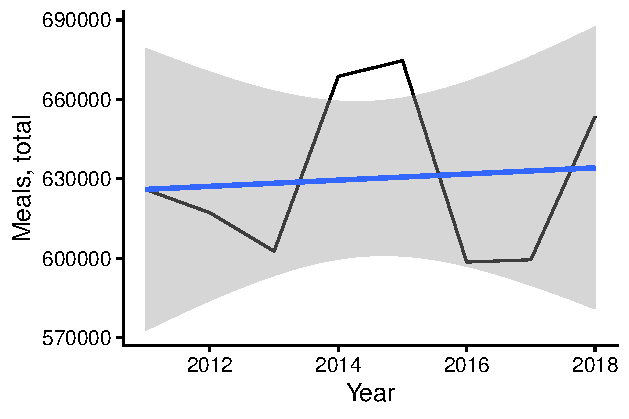
\includegraphics[width=\maxwidth]{figure/beamer-FundamentalDynamicsMealsTotal-1} 

}



\end{frame}

\begin{frame}[fragile]
\frametitle{Dynamik der Fördersumme, Mittagstisch: Median}



{\centering 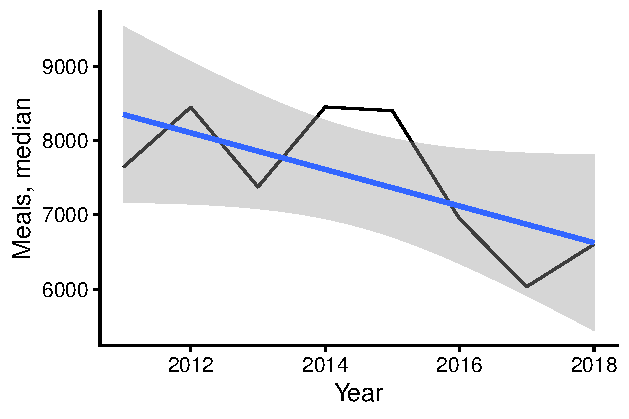
\includegraphics[width=\maxwidth]{figure/beamer-FundamentalDynamicsMealsMedian-1} 

}



\end{frame}

\begin{frame}[fragile]
\frametitle{Dynamik der Fördersumme, Mittagstisch: Median pro Begünstigter}


{\centering 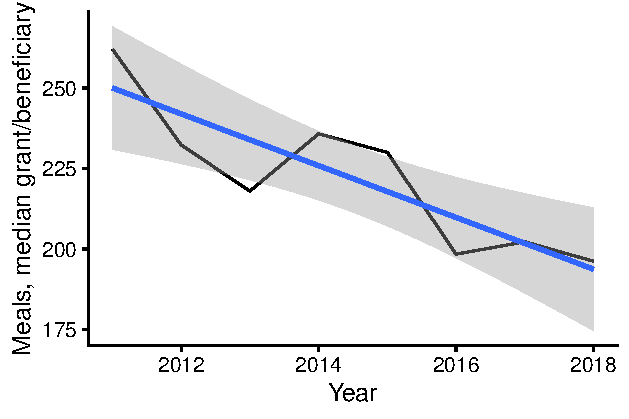
\includegraphics[width=\maxwidth]{figure/beamer-FundamentalDynamicsMealsMedianPerBene-1} 

}



\end{frame}

\begin{frame}[fragile]
\frametitle{Dynamik der Fördersumme, Entdeckerfonds: Summe}



{\centering 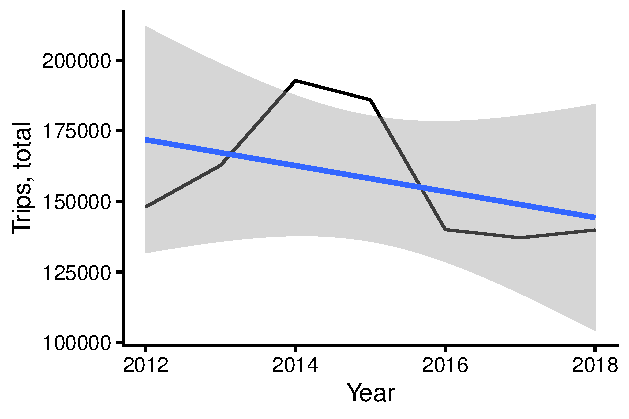
\includegraphics[width=\maxwidth]{figure/beamer-FundamentalDynamicsTripsTotal-1} 

}



\end{frame}

\begin{frame}[fragile]
\frametitle{Dynamik der Fördersumme, Entdeckerfonds: Median}



{\centering 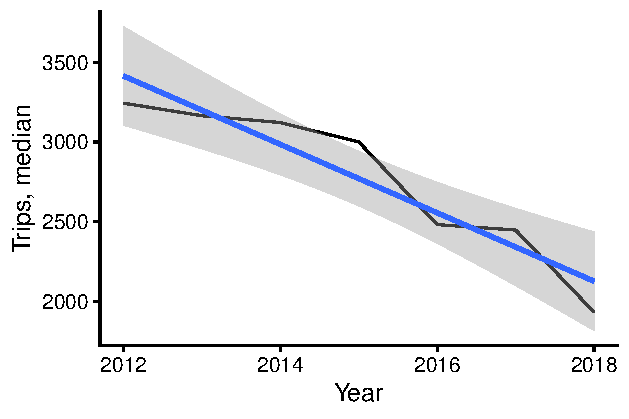
\includegraphics[width=\maxwidth]{figure/beamer-FundamentalDynamicsTripsMedian-1} 

}



\end{frame}

\begin{frame}[fragile]
\frametitle{Dynamik der Fördersumme, Entdeckerfonds: Median pro Begünstigter}


{\centering 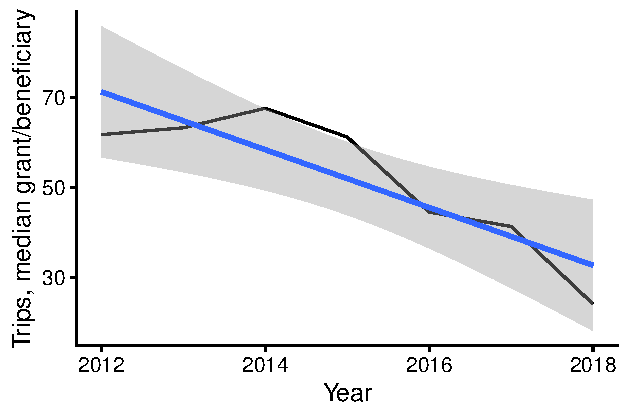
\includegraphics[width=\maxwidth]{figure/beamer-FundamentalDynamicsTripsMedianPerBene-1} 

}



\end{frame}

\subsection{Dynamiken des Selbstwertgefühls und der Alltagskompetenzen}

\begin{frame}[fragile]
\frametitle{Variable "Selbstwertgefühl": Dynamik}
\begin{knitrout}\footnotesize
\definecolor{shadecolor}{rgb}{0.969, 0.969, 0.969}\color{fgcolor}

{\centering 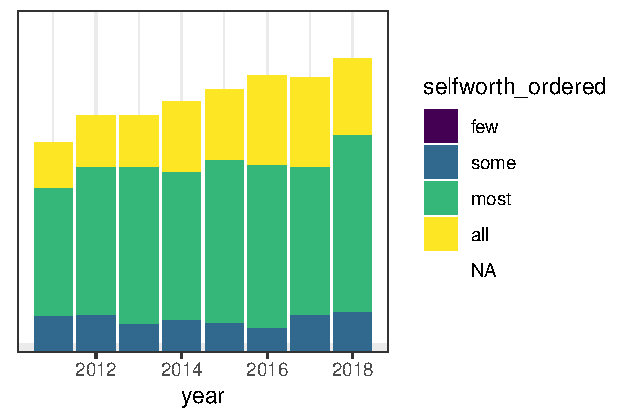
\includegraphics[width=\maxwidth]{figure/beamer-SelfworthTime-1} 

}



\end{knitrout}
\end{frame}

\begin{frame}[fragile]
\frametitle{Variable "Alltagskompetenzen": Dynamik}
\begin{knitrout}\footnotesize
\definecolor{shadecolor}{rgb}{0.969, 0.969, 0.969}\color{fgcolor}

{\centering 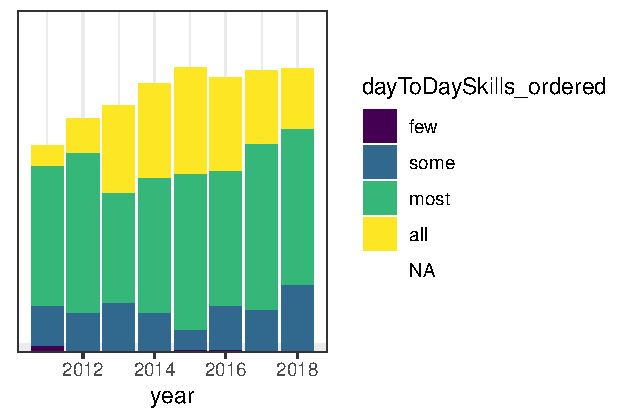
\includegraphics[width=\maxwidth]{figure/beamer-DayToDayTime-1} 

}



\end{knitrout}
\end{frame}

\subsection{Dynamiken der gesundheitsrelevanten Variablen}

\begin{frame}[fragile]
\frametitle{Variable "seltener krank": Dynamik}
\begin{knitrout}\footnotesize
\definecolor{shadecolor}{rgb}{0.969, 0.969, 0.969}\color{fgcolor}

{\centering 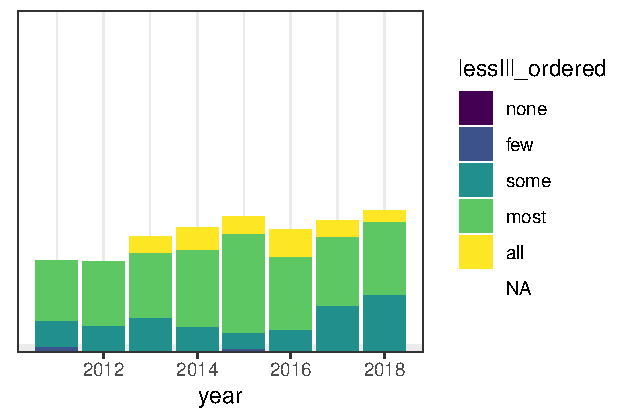
\includegraphics[width=\maxwidth]{figure/beamer-lessIllTime-1} 

}



\end{knitrout}
\end{frame}

\begin{frame}[fragile]
\frametitle{Variable "Wertschätzung gesunder Ernährung": Dynamik}

\begin{knitrout}\footnotesize
\definecolor{shadecolor}{rgb}{0.969, 0.969, 0.969}\color{fgcolor}\begin{kframe}


{\ttfamily\noindent\color{warningcolor}{\#\# Warning in gzfile(file, "{}rb"{}): kann komprimierte Datei './ANALYSIS/GRAPHS/PAPER/appreciate\_Time.Rds.Rds' nicht öffnen. Grund evtl. 'No such file or directory'}}

{\ttfamily\noindent\bfseries\color{errorcolor}{\#\# Error in gzfile(file, "{}rb"{}): kann Verbindung nicht öffnen}}

{\ttfamily\noindent\bfseries\color{errorcolor}{\#\# Error in print(appreciatetimeplot, label = "{}lessilltimeplot"{}): Objekt 'appreciatetimeplot' nicht gefunden}}\end{kframe}
\end{knitrout}
\end{frame}

\begin{frame}[fragile]
\frametitle{Dynamics}

\begin{figure}
  \caption{Yearly dynamics of total grants in Meals and Trips program}
  \label{totalGrantsDyn}
  
\begin{knitrout}\footnotesize
\definecolor{shadecolor}{rgb}{0.969, 0.969, 0.969}\color{fgcolor}

{\centering 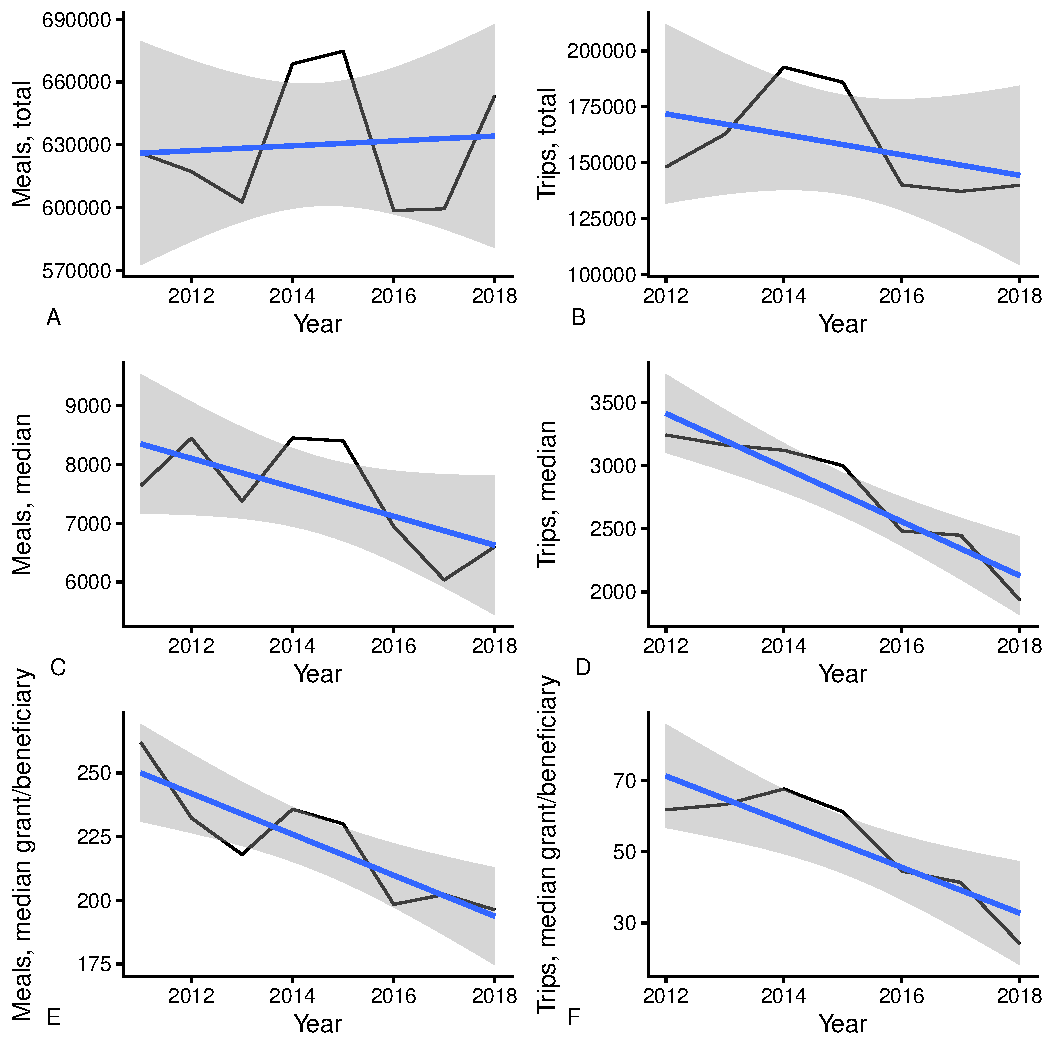
\includegraphics[width=\maxwidth]{figure/beamer-GrantTrend-1} 

}



\end{knitrout}

% \floatfoot{This graph shows the development of grants in the Meals compared to the Trips program. We distinguish between the sum of grants in one year, the median grant and the median grant per beneficiary. From left to right: Meals, Trips. From top to bottom: sum, median, median per beneficiary. We have deflated the values to 2015 euros using the price index related to food and non-alcoholic beverages(in German: Nahrungsmittel und alkoholfreie Getränke) for the Meals program and the price index related to Leisure, Entertainment and Culture (in German: Freizeit, Unterhaltung, Kultur) provided by the Federal Statistical Office of Germany (Statistisches Bundesamt).}
\end{figure}

\end{frame}


\section[Zusammenhang Zuschüsse \& ausgewählte Variablen]{Zusammenhang zwischen CHILDRENs Zuschüssen und ausgewählten Variablen}

\begin{frame}
\frametitle{Empirischer Ansatz}
\begin{equation}
\label{SimpleLinearModel}
  y_{it} = \beta_0 + \beta_1 x_{it} + \epsilon_{it}
\end{equation}
\end{frame}

\subsection{Direkte Effekte von CHILDRENs Zuschüssen} 

\begin{frame}[fragile]
\frametitle{Zusammenhang Mahlzeiten und Zuschüsse}


\begin{table}
\caption{Zusammenhang zwischen Anzahl der Mahlzeiten und realer Fördersumme}
\begin{center}
\scalebox{0.5}{
\begin{tabular}{l c c c c c }
\toprule
 & (1) & (2) & (3) & (4) & (5) \\
\midrule
(Intercept)     & $-12089.14^{*}$ & $-1814.16$     & $3535.39^{***}$ & $3107.70^{***}$ & $-12250.60^{**}$ \\
                & $(5192.86)$     & $(1765.93)$    & $(498.99)$      & $(508.94)$      & $(4524.09)$      \\
realSubsidy     & $2.61^{***}$    & $0.50^{**}$    & $0.29^{***}$    & $0.25^{***}$    & $2.72^{***}$     \\
                & $(0.57)$        & $(0.18)$       & $(0.05)$        & $(0.05)$        & $(0.51)$         \\
eatersPerMealNo &                 & $172.83^{***}$ &                 & $19.00^{*}$     &                  \\
                &                 & $(14.92)$      &                 & $(8.45)$        &                  \\
\midrule
R$^2$           & 0.43            & 0.73           & 0.13            & 0.21            & 0.45             \\
Adj. R$^2$      & 0.43            & 0.73           & 0.12            & 0.20            & 0.45             \\
Num. obs.       & 329             & 329            & 250             & 250             & 440              \\
RMSE            & 39992.79        & 27390.90       & 3629.72         & 3463.66         & 39601.41         \\
\bottomrule
\multicolumn{6}{l}{\scriptsize{\parbox{\linewidth}
{\vspace{2pt} Abhängige Variable: Anzahl der Mahlzeiten \\ realSubsidy: Fördersumme für Mittagstisch (EUR von 2015)\\ eatersPerMeal: Anzahl der durch Mittagtisch Begünstigten, einfaches lineares Modell, geschätzt mit Ansatz der kleinsten Quadrate \\ Modell (2): ursprünglicher Datensatz, lineares Modell mit Kontrollen, geschätzt mit Ansatz der kleinsten Quadrate \\ Modell (3): Datensatz ohne Ausreißer, einfaches lineares Modell, geschätzt mit Ansatz der kleinsten Quadrate \\ Modell (4): data set without outliers, linear model with controls, estimated with OLS \\ Model (5): imputed data set, simple linear model, estimated with OLS \\ All regressions are estimated with robust standard errors $^{***}p<0.001$, $^{**}p<0.01$, $^*p<0.05$.}}}
\end{tabular}
}
\label{GrantsRegressionsLunch}
\end{center}
\end{table}

\end{frame}

\begin{frame}[fragile]
\frametitle{Zusammenhang Ausflüge und Zuschüsse}

\begin{table}
\caption{Association between number of trips and real subsidy}
\begin{center}
\scalebox{0.8}{
\begin{tabular}{l c c c c c }
\toprule
 & (1) & (2) & (3) & (4) & (5) \\
\midrule
(Intercept)      & $3.7049^{***}$ & $3.4394^{***}$ & $2.6236^{***}$ & $2.3660^{***}$ & $3.6237^{***}$ \\
                 & $(0.3313)$     & $(0.3359)$     & $(0.2300)$     & $(0.2609)$     & $(0.3253)$     \\
realTripsSubsidy & $0.0002^{*}$   & $0.0001$       & $0.0003^{***}$ & $0.0003^{***}$ & $0.0002^{*}$   \\
                 & $(0.0001)$     & $(0.0001)$     & $(0.0001)$     & $(0.0001)$     & $(0.0001)$     \\
tripsKidsNo      &                & $0.0059$       &                & $0.0043$       &                \\
                 &                & $(0.0032)$     &                & $(0.0027)$     &                \\
\midrule
R$^2$            & 0.0474         & 0.0729         & 0.0880         & 0.1241         & 0.0504         \\
Adj. R$^2$       & 0.0444         & 0.0671         & 0.0844         & 0.1172         & 0.0476         \\
Num. obs.        & 322            & 319            & 257            & 256            & 334            \\
RMSE             & 2.9565         & 2.8967         & 1.6981         & 1.6579         & 2.9310         \\
\bottomrule
\multicolumn{6}{l}{\scriptsize{\parbox{\linewidth}
{\vspace{2pt} Dependent variable: number of trips \\ realTripsSubsidy: subsidy for Trips program in 2015 EUR \\ tripsKidsNo: number of beneficiaries of Trips program \\ Model (1): original data set, simple linear model, estimated with OLS \\ Model (2): original data set, linear model with controls, estimated with OLS \\ Model (3): data set without outliers, simple linear model, esmitaed with OLS \\ Model (4): data set without outliers, linear model with controls, estimated with OLS \\ Model (5): imputed data set, simple linear model, estimated with OLS \\ All regressions are estimated with robust standard errors $^{***}p<0.001$, $^{**}p<0.01$, $^*p<0.05$.}}}
\end{tabular}
}
\label{GrantsRegressionsTrips}
\end{center}
\end{table}

\end{frame}

\subsection{Selbstwertgefühl, Alltagskompetenzen und Zuschüsse}

\begin{frame}[fragile]
\frametitle{Selbstwertgefühl}


\begin{table}
\caption{Association between selfworth and subsidy per beneficiary}
\begin{center}
\scalebox{0.8}{
\begin{tabular}{l c c c c c }
\hline
 & (1) & (2) & (3) & (4) & (5) \\
\hline
(Intercept)                    & $0.08$   & $0.12$   & $0.09$   & $0.12$   & $0.23^{*}$   \\
                               & $(0.09)$ & $(0.12)$ & $(0.09)$ & $(0.11)$ & $(0.11)$     \\
realSubsidyPerBeneficiary      & $-0.00$  &          & $-0.00$  &          & $-0.00$      \\
                               & $(0.00)$ &          & $(0.00)$ &          & $(0.00)$     \\
realTripsSubsidyPerBeneficiary &          & $-0.00$  &          & $-0.00$  &              \\
                               &          & $(0.00)$ &          & $(0.00)$ &              \\
ML1                            &          &          &          &          & $0.24^{***}$ \\
                               &          &          &          &          & $(0.06)$     \\
ML2                            &          &          &          &          & $0.37^{***}$ \\
                               &          &          &          &          & $(0.05)$     \\
ML3                            &          &          &          &          & $0.15^{***}$ \\
                               &          &          &          &          & $(0.04)$     \\
\hline
R$^2$                          & 0.00     & 0.01     & 0.00     & 0.01     & 0.30         \\
Adj. R$^2$                     & 0.00     & 0.01     & 0.00     & 0.01     & 0.28         \\
Num. obs.                      & 428      & 184      & 430      & 187      & 161          \\
RMSE                           & 1.00     & 1.00     & 1.00     & 1.00     & 0.79         \\
\hline
\multicolumn{6}{l}{\scriptsize{\parbox{\linewidth}
{\vspace{2pt} realSubsidyPerBeneficiary: subsidy per beneficiary of Meals program in 2015 EUR \\ realTripsSubsidyPerBeneficiary: subsidy per beneficiary of Trips program in 2015 EUR \\Model (1): dependent variable: share of beneficiaries with improved self-worth in the Lunch program, original data set, simple linear model, estimated with OLS \\ Model (2): dependent variable: share of beneficiaries with improved self-worth in the Trips program, original data set, simple linear model, estimated with OLS \\ Model (3): dependent variable: share of beneficiaries with improved self-worth in the Lunch program, imputed data set, simple linear model, estimated with OLS \\ Model (4): dependent variable: share of beneficiaries with improved self-worth in the Trips program, imputed data set, simple linear model, estimated with OLS \\ Model (5): dependent variable: share of beneficiaries with improved self-worth in the Lunch program, imputed data set, linear model with extracted factor scores as controls, estimated with OLS \\ All regressions are estimated with robust standard errors $^{***}p<0.001$, $^{**}p<0.01$, $^*p<0.05$.}}}
\end{tabular}
}
\label{SelfworthRegressions}
\end{center}
\end{table}


\end{frame}

\begin{frame}[fragile]
\frametitle{Alltagskompetenzen}


\begin{table}
\caption{Association between everyday expertise and subsidy per beneficiary}
\begin{center}
\scalebox{0.8}{
\begin{tabular}{l c c c c c c }
\hline
 & (1) & (2) & (3) & (4) & (5) & (6) \\
\hline
(Intercept)                    & $0.15$   & $0.13$   & $0.14$   & $0.11$   & $0.28^{*}$   & $0.08$       \\
                               & $(0.09)$ & $(0.10)$ & $(0.09)$ & $(0.10)$ & $(0.11)$     & $(0.09)$     \\
realSubsidyPerBeneficiary      & $-0.00$  &          & $-0.00$  &          & $-0.00$      &              \\
                               & $(0.00)$ &          & $(0.00)$ &          & $(0.00)$     &              \\
realTripsSubsidyPerBeneficiary &          & $-0.00$  &          & $-0.00$  &              & $-0.00$      \\
                               &          & $(0.00)$ &          & $(0.00)$ &              & $(0.00)$     \\
ML1                            &          &          &          &          & $0.31^{***}$ & $0.03$       \\
                               &          &          &          &          & $(0.06)$     & $(0.07)$     \\
ML2                            &          &          &          &          & $0.40^{***}$ & $0.16^{*}$   \\
                               &          &          &          &          & $(0.06)$     & $(0.07)$     \\
ML3                            &          &          &          &          & $0.16^{**}$  & $0.19^{**}$  \\
                               &          &          &          &          & $(0.05)$     & $(0.06)$     \\
ML4                            &          &          &          &          &              & $0.49^{***}$ \\
                               &          &          &          &          &              & $(0.06)$     \\
\hline
R$^2$                          & 0.01     & 0.01     & 0.01     & 0.01     & 0.37         & 0.37         \\
Adj. R$^2$                     & 0.01     & 0.01     & 0.01     & 0.01     & 0.36         & 0.35         \\
Num. obs.                      & 426      & 177      & 429      & 181      & 161          & 169          \\
RMSE                           & 1.00     & 0.98     & 1.00     & 0.99     & 0.78         & 0.80         \\
\hline
\multicolumn{7}{l}{\scriptsize{\parbox{\linewidth}
{\vspace{2pt} realSubsidyPerBeneficiary: subsidy per beneficiary of Meals program in 2015 EUR \\ realTripsSubsidyPerBeneficiary: subsidy per beneficiary of Trips program in 2015 EUR \\ Model (1): dependent variable: share of beneficiaries with with broadened everyday expertise in the Lunch program, original data set, simple linear model, estimated with OLS \\ Model (2): dependent variable: share of beneficiaries with with broadened everyday expertise in the Trips program, original data set, simple linear model, estimated with OLS \\ Model (3): dependent variable: share of beneficiaries with with broadened everyday expertise in the Lunch program, imputed data set, simple linear model, estimated with OLS \\ Model (4): dependent variable: share of beneficiaries with with broadened everyday expertise in the Trips program, imputed data set, simple linear model, estimated with OLS\\ Model (5): dependent variable: share of beneficiaries with with broadened everyday expertise in the Lunch program, imputed data set, linear model with extracted factor scores as controls, estimated with OLS \\ Model (6): dependent variable: share of beneficiaries with with broadened everyday expertise in the Trips program, imputed data set, linear model with extracted factor scores as controls, estimated with OLS \\ All regressions are estimated with robust standard errors $^{***}p<0.001$, $^{**}p<0.01$, $^*p<0.05$.}}}
\end{tabular}
}
\label{DayToDaySkillsRegressions}
\end{center}
\end{table}


\end{frame}

\subsection{Gesundheit}

\begin{frame}[fragile]
\frametitle{Seltener krank}

\begin{table}
\caption{Association between healthy meals criterion and beneficiaries being less ill}
\begin{center}
\scalebox{0.8}{
\begin{tabular}{l c c c c c }
\hline
 & (1) & (2) & (3) & (4) & (5) \\
\hline
(Intercept)         & $0.02$       & $0.46^{**}$ & $0.09$       & $0.39^{***}$ & $0.05$       \\
                    & $(0.08)$     & $(0.16)$    & $(0.07)$     & $(0.12)$     & $(0.07)$     \\
DGECriteriaNoScaled & $0.33^{***}$ & $0.35^{*}$  & $0.25^{***}$ & $0.24$       & $0.18^{*}$   \\
                    & $(0.08)$     & $(0.16)$    & $(0.07)$     & $(0.14)$     & $(0.07)$     \\
ML1                 &              &             &              &              & $0.12^{*}$   \\
                    &              &             &              &              & $(0.06)$     \\
ML2                 &              &             &              &              & $0.27^{***}$ \\
                    &              &             &              &              & $(0.06)$     \\
\hline
R$^2$               & 0.12         & 0.29        & 0.07         & 0.16         & 0.19         \\
Adj. R$^2$          & 0.11         & 0.29        & 0.07         & 0.16         & 0.17         \\
Num. obs.           & 121          & 120         & 177          & 177          & 161          \\
RMSE                & 0.91         & 7.83        & 0.94         & 7.95         & 0.87         \\
\hline
\multicolumn{6}{l}{\scriptsize{\parbox{\linewidth}
{\vspace{2pt} Dependent variable: share of beneficiaries who are less frequently ill \\ DGECriteriaNo: index of healthy diet criteria fulfilled in organization's menu \\ Model (1): original data set, simple linear model, estimated with OLS \\ Model (2): original data set, simple linear model, estimated with WLS \\ Model (3): imputed data set, simple linear model, estimated with OLS \\ Model (4): imputed data set, simple linear model, estimated with WLS \\ Model (5): imputed data set, linear model with extracted factor scores as controls, estimated with OLS \\ All regressions are estimated with robust standard errors $^{***}p<0.001$, $^{**}p<0.01$, $^*p<0.05$.}}}
\end{tabular}
}
\label{HealthRegressions-LessIll}
\end{center}
\end{table}

\end{frame}

\begin{frame}
\frametitle{Ernährungswissen}

\begin{table}
\caption{Association between healthy meals criterion and beneficiaries dietary knowledge}
\begin{center}
\scalebox{0.8}{
\begin{tabular}{l c c c c c }
\hline
 & (1) & (2) & (3) & (4) & (5) \\
\hline
(Intercept)         & $0.02$   & $0.08$   & $0.02$     & $0.21$   & $0.02$       \\
                    & $(0.07)$ & $(0.19)$ & $(0.06)$   & $(0.18)$ & $(0.07)$     \\
DGECriteriaNoScaled & $0.11$   & $-0.02$  & $0.12^{*}$ & $0.10$   & $-0.00$      \\
                    & $(0.06)$ & $(0.12)$ & $(0.05)$   & $(0.14)$ & $(0.06)$     \\
ML1                 &          &          &            &          & $0.26^{***}$ \\
                    &          &          &            &          & $(0.06)$     \\
ML2                 &          &          &            &          & $0.24^{***}$ \\
                    &          &          &            &          & $(0.06)$     \\
ML3                 &          &          &            &          & $0.37^{***}$ \\
                    &          &          &            &          & $(0.06)$     \\
\hline
R$^2$               & 0.01     & 0.00     & 0.02       & 0.01     & 0.31         \\
Adj. R$^2$          & 0.01     & -0.00    & 0.01       & 0.01     & 0.29         \\
Num. obs.           & 214      & 212      & 275        & 275      & 161          \\
RMSE                & 0.98     & 8.49     & 0.96       & 9.45     & 0.83         \\
\hline
\multicolumn{6}{l}{\scriptsize{\parbox{\linewidth}
{\vspace{2pt} Dependent variable: share of beneficiaries with expanded dietary knowledge \\ DGECriteriaNo: index of healthy diet criteria fulfilled in organization's menu \\ Model (1): original data set, simple linear model, estimated with OLS \\ Model (2): original data set, simple linear model, estimated with WLS \\ Model (3): imputed data set, simple linear model, estimated with OLS \\ Model (4): imputed data set, simple linear model, estimated with WLS \\ Model (5): imputed data set, linear model with extracted factor scores as controls, estimated with OLS \\ All regressions are estimated with robust standard errors $^{***}p<0.001$, $^{**}p<0.01$, $^*p<0.05$.}}}
\end{tabular}
}
\label{HealthRegressions-DietaryKnowledge}
\end{center}
\end{table}

\end{frame}

\begin{frame}[fragile]
\frametitle{Wertschätzung für gesundes Essen}

\begin{table}
\caption{Association between healthy meals criterion and  beneficiaries appreciation of a healthy diet}
\begin{center}
\scalebox{0.8}{
\begin{tabular}{l c c c c c }
\hline
 & (1) & (2) & (3) & (4) & (5) \\
\hline
(Intercept)         & $-0.03$      & $0.26$   & $0.02$       & $0.37^{*}$ & $0.05$       \\
                    & $(0.07)$     & $(0.18)$ & $(0.06)$     & $(0.17)$   & $(0.07)$     \\
DGECriteriaNoScaled & $0.27^{***}$ & $-0.02$  & $0.25^{***}$ & $0.01$     & $0.03$       \\
                    & $(0.07)$     & $(0.15)$ & $(0.06)$     & $(0.13)$   & $(0.06)$     \\
ML1                 &              &          &              &            & $0.03$       \\
                    &              &          &              &            & $(0.07)$     \\
ML2                 &              &          &              &            & $0.47^{***}$ \\
                    &              &          &              &            & $(0.05)$     \\
ML3                 &              &          &              &            & $0.24^{***}$ \\
                    &              &          &              &            & $(0.05)$     \\
\hline
R$^2$               & 0.06         & 0.00     & 0.06         & 0.00       & 0.37         \\
Adj. R$^2$          & 0.06         & -0.00    & 0.06         & -0.00      & 0.35         \\
Num. obs.           & 213          & 211      & 274          & 274        & 161          \\
RMSE                & 1.02         & 8.61     & 1.01         & 9.00       & 0.82         \\
\hline
\multicolumn{6}{l}{\scriptsize{\parbox{\linewidth}
{\vspace{2pt} Dependent variable: share of beneficiaries with increased appreciation for a healthy diet \\ DGECriteriaNo: index of healthy diet criteria fulfilled in organization's menu \\ Model (1): original data set, simple linear model, estimated with OLS \\ Model (2): original data set, simple linear model, estimated with WLS \\ Model (3): imputed data set, simple linear model, estimated with OLS \\ Model (4): imputed data set, simple linear model, estimated with WLS \\ Model (5): imputed data set, linear model with extracted factor scores as controls, estimated with OLS \\ All regressions are estimated with robust standard errors $^{***}p<0.001$, $^{**}p<0.01$, $^*p<0.05$.}}}
\end{tabular}
}
\label{HealthRegressions-AppreciateHealthy}
\end{center}
\end{table}

\end{frame}

\section{Partition}

\begin{frame}[fragile]
\frametitle{Partition Mittagstisch}
% latex table generated in R 3.6.2 by xtable 1.8-4 package
% Sun Mar 01 20:37:09 2020
\begin{table}[ht]
\centering
\begin{tabular}{lccc}
  \hline
 & Variable, Meals & Mapping, Meals & Information, Meals \\ 
  \hline
1 & participateMore & participateMore & 1.00 \\ 
  2 & tasksLunch & tasksLunch & 1.00 \\ 
  3 & ownIdeas & ownIdeas & 1.00 \\ 
  4 & stayLonger & stayLonger & 1.00 \\ 
  5 & dietaryKnowledge & dietaryKnowledge & 1.00 \\ 
  6 & appreciateHealthy & appreciateHealthy & 1.00 \\ 
  7 & foodCulture & foodCulture & 1.00 \\ 
  8 & lessIll & lessIll & 1.00 \\ 
  9 & betterTeamwork & betterTeamwork & 1.00 \\ 
  10 & moreRegularSchoolVisits & moreRegularSchoolVisits & 1.00 \\ 
  11 & addressProblems & addressProblems & 1.00 \\ 
  12 & reduced\_var\_1 & moreConcentrated & 0.66 \\ 
  13 & reduced\_var\_1 & moreBalanced & 0.66 \\ 
  14 & reduced\_var\_2 & monthlyCooks & 0.42 \\ 
  15 & reduced\_var\_2 & weeklyCooks & 0.42 \\ 
  16 & reduced\_var\_2 & shoppers & 0.42 \\ 
  17 & reduced\_var\_2 & easyDishes & 0.42 \\ 
  18 & reduced\_var\_3 & dayToDaySkills & 0.43 \\ 
  19 & reduced\_var\_3 & moreIndependent & 0.43 \\ 
  20 & reduced\_var\_3 & selfworth & 0.43 \\ 
  21 & reduced\_var\_3 & moreOpen & 0.43 \\ 
  22 & reduced\_var\_3 & moreConfidence & 0.43 \\ 
  23 & reduced\_var\_3 & proud & 0.43 \\ 
  24 & reduced\_var\_4 & betterReading & 0.53 \\ 
  25 & reduced\_var\_4 & betterNumbers & 0.53 \\ 
  26 & reduced\_var\_4 & betterGrades & 0.53 \\ 
  27 & reduced\_var\_5 & influenceHome & 0.41 \\ 
  28 & reduced\_var\_5 & cookAtHome & 0.41 \\ 
  29 & reduced\_var\_5 & askRecipes & 0.41 \\ 
   \hline
\end{tabular}
\caption{Partition of outcomes, Meals} 
\label{partitionmeals}
\end{table}


\end{frame}

\begin{frame}
\frametitle{Partition Entdeckerfonds}
% latex table generated in R 3.6.2 by xtable 1.8-4 package
% Sun Mar 01 20:37:09 2020
\begin{table}[ht]
\centering
\begin{tabular}{lccc}
  \hline
 & Variable, Trips & Mapping, Trips & Information, Trips \\ 
  \hline
1 & tripsSuggestions & tripsSuggestions & 1.00 \\ 
  2 & tripsDecisions & tripsDecisions & 1.00 \\ 
  3 & tripsOrganization & tripsOrganization & 1.00 \\ 
  4 & tripsCostCalculation & tripsCostCalculation & 1.00 \\ 
  5 & tripsBudget & tripsBudget & 1.00 \\ 
  6 & tripsMoney & tripsMoney & 1.00 \\ 
  7 & tripsReview & tripsReview & 1.00 \\ 
  8 & tripsPublicTransport & tripsPublicTransport & 1.00 \\ 
  9 & tripsMobility & tripsMobility & 1.00 \\ 
  10 & tripsAdditionalActivities & tripsAdditionalActivities & 1.00 \\ 
  11 & tripsSelfworth & tripsSelfworth & 1.00 \\ 
  12 & tripsFrustrationTolerance & tripsFrustrationTolerance & 1.00 \\ 
  13 & reduced\_var\_1 & tripsSuccess & 0.68 \\ 
  14 & reduced\_var\_1 & tripsSelfEfficacy & 0.68 \\ 
  15 & reduced\_var\_2 & tripsNewPlaces & 0.60 \\ 
  16 & reduced\_var\_2 & tripsNewCommunities & 0.60 \\ 
  17 & reduced\_var\_2 & tripsNewIdeas & 0.60 \\ 
  18 & reduced\_var\_2 & tripsSocialSkills & 0.60 \\ 
  19 & reduced\_var\_3 & tripsSpecificSkills & 0.46 \\ 
  20 & reduced\_var\_3 & tripsDayToDaySkills & 0.46 \\ 
   \hline
\end{tabular}
\caption{Partition of outcomes, Trips} 
\label{partitiontrips}
\end{table}

\end{frame}

\section{Effekte des Entdeckerfonds}

\subsection{Idee}

\begin{frame}[fragile]
\frametitle{Idee}
\end{frame}

\subsection{Empirische Methode}

\begin{frame}[fragile]
\frametitle{Definition der Treatmentgruppe}
\end{frame}

\begin{frame}[fragile]
\frametitle{Zielvariable}
\end{frame}

\begin{frame}[fragile]
\frametitle{Graphische Darstellung: Alltagskompetenzen}
\end{frame}

\begin{frame}[fragile]
\frametitle{Graphische Darstellung: Selbstwertgefühl}
\end{frame}

\begin{frame}[fragile]
\frametitle{DID - Schätzung}
\end{frame}

\subsection{Ergebnisse}

\begin{frame}[fragile]
\frametitle{Alltagskompetenzen}
\end{frame}

\begin{frame}[fragile]
\frametitle{Selbstwertgefühl}
\end{frame}

\frame[allowframebreaks]{\frametitle{References}
		\tiny
		\printbibliography
}
	
\end{document}


